\documentclass[11pt]{article}
\usepackage[utf8]{inputenc}	% Para caracteres en español
\usepackage{amsmath,amsthm,amsfonts,amssymb,amscd}
\usepackage{multirow,booktabs}
\usepackage[table]{xcolor}
\usepackage{fullpage}
\usepackage{lastpage}
\usepackage{enumitem}
\usepackage{fancyhdr}
\usepackage{mathrsfs}
\usepackage{wrapfig}
\usepackage{setspace}
\usepackage{calc}
\usepackage{multicol}
\usepackage{cancel}
\usepackage{float}
\usepackage{physics}
\usepackage[retainorgcmds]{IEEEtrantools}
\usepackage[margin=1cm]{geometry}
\usepackage{amsmath}
\newlength{\tabcont}
\setlength{\parindent}{0.0in}
\setlength{\parskip}{0.05in}
\setlength{\headheight}{14pt}
\usepackage{empheq}
\usepackage{framed}
\usepackage[most]{tcolorbox}
\usepackage{xcolor}
\usepackage[version=3]{mhchem}
\usepackage[english]{babel}
\usepackage[utf8]{inputenc}
\usepackage{graphicx}
\usepackage[colorinlistoftodos]{todonotes}
\usepackage{mdframed}

\colorlet{shadecolor}{orange!15}
\parindent 0in
\parskip 12pt
\geometry{margin=1in, headsep=0.25in}
\theoremstyle{definition}
\newtheorem{defn}{Definition}
\newtheorem{reg}{Rule}
\newtheorem{exer}{Exercise}
\newtheorem{note}{Note}
\begin{document}
\setcounter{section}{2}
%\setcounter{subsection}{}
\title{Midterms}

%==============================================================
%\thispagestyle{empty}
\pagestyle{fancy}
\fancyhf{}
\rhead{Physics 180}
\chead{Midterms}
\lhead{Olyn D. Desabelle}
\rfoot{Page \thepage}

\begin{center}
{\LARGE \bf Midterms}\\
%{\large Physics 180}\\
%Olyn D. Desabelle
\end{center}

\begin{mdframed}
    I swear upon my honor that I have not given nor received any unauthorized help on this exam and that all the work below are my own.
\end{mdframed}
\begin{figure}[H]
    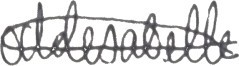
\includegraphics[scale = 20]{my e-sig.jpg}
\end{figure}

DESABELLE, Olyn D.

\noindent\makebox[\linewidth]{\rule{\paperwidth}{0.4pt}}



\begin{figure}[H]
    \centering
    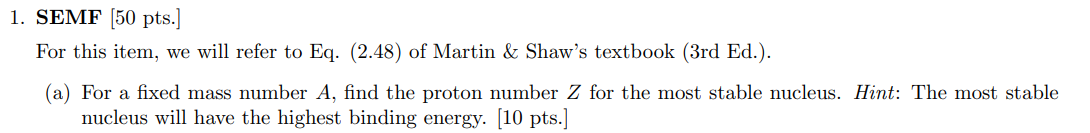
\includegraphics[scale = 0.5]{1a.png}
\end{figure}

Equation (2.48) of Martin \& Shaw gives the mass deficit $\Delta M(Z,A)$:

\begin{align*}
    \Delta M(Z,A) \equiv M(Z,A) - Z(M_p + m_e) - NM_n
    \tag*{(2.48)}
\end{align*}

we note that the first term of the RHS of Equation (2.48) is given by Equation (2.49)

\begin{align*}
    \text{M}(\text{Z},\text{A}) = \sum_{i=0}^{5} f_i(\text{Z},\text{A}) \tag{2.49}
\end{align*}

where each $f_i(\text{Z},\text{A})$ is given by Equations (2.50-2.55):

\begin{align*}
    f_0(\text{Z},\text{A}) &= \text{Z}(M_p + m_e) + (\text{A}-\text{Z})M_n \tag{2.50}\\
    f_1(\text{Z},\text{A}) &= -a_v  A \tag{2.51}\\
    f_2(\text{Z},\text{A}) &= a_s A^{2/3} \tag{2.52}\\
    %f_3(\text{Z},\text{A}) &= a_c \frac{Z(Z-1)}{A^{1/3}} \tag{2.53}\\
    f_3(\text{Z},\text{A}) &= a_c \frac{Z(Z-1)}{A^{1/3}} \tag{2.53}\\
    f_4(\text{Z},\text{A}) &= a_a \frac{(Z-A/2)^2}{A} \tag{2.54}\\
    f_5(\text{Z},\text{A}) &= -f(A)\;\;\; \text{if both } Z,N \text{ are even} \\
    &= +f(A)\;\;\; \text{if both } Z,N \text{ are odd} \tag{2.55}\\
    &= 0 \;\;\; \text{ if either one of } Z,N \text{ is odd and the other is even } \\
\end{align*}

\begin{align*}
    a_v = 15.56,\;\;\; a_s = 17.23,\;\;\; a_c = 0.697,\;\;\; a_a = 93.14 \;\;\; a_p = 12
\end{align*}

where $N=A-Z$, $f(A) = a_p A^{-1/2}$, and the $a_i$ coefficients are in units of $\text{MeV}/c^2$. We may plug these into Equation (2.48), from which we may get the binding energy $B$ from:

\begin{align}
    B = - \Delta Mc^2
\end{align}

rewriting the conditions for $f_5$ in terms of $A$ and $Z$, we thus have:

\begin{align}
    B &= 
    \begin{cases}
        -a_v  A + a_s A^{2/3} + a_c \frac{Z(Z-1)}{A^{1/3}} + a_a\frac{(Z-A/2)^2}{A} + a_p A^{-1/2} & \text{ for even } A,\text{ odd Z}\\
        %\text{ if both }Z,N \text{ are odd}\\
        -a_v  A + a_s A^{2/3} + a_c \frac{Z(Z-1)}{A^{1/3}} + a_a\frac{(Z-A/2)^2}{A} - a_p A^{-1/2} & \text{ for even }A,\text{ even Z}\\
        %\text{ if both }Z,N \text{ are even}\\
        -a_v  A + a_s A^{2/3} + a_c \frac{Z(Z-1)}{A^{1/3}} + a_a\frac{(Z-A/2)^2}{A} & \text{ for odd }A
    \end{cases}
\end{align}

to get the highest binding energy $B$ for the most stable nucleus given $A$, we get its derivative with respect to $Z$:

\begin{align}
    \frac{dB}{dZ} &= 
        a_c \frac{2Z-1}{A^{1/3}} +a_a \frac{2Z-A}{A}
\end{align}

at the maxima, $\frac{dB}{dZ} = 0$ and thus we have the relation:

\begin{align}
    0 = 
    a_c \frac{2Z-1}{A^{1/3}} +a_a \frac{2Z-A}{A}\\
    A^{2/3}a_c(2Z-1) + a_a(2Z-A) = 0
\end{align}

\begin{equation}\label{za}
\boxed{
    Z = \frac{A^{2/3}a_c + Aa_a}{2a_a + 2A^{2/3}a_c}
}
\end{equation}

%\begin{align} Z =
%\begin{cases}
%    \frac{-a_v  A^2 + a_s A^{5/3} - a_c A^{2/3} -A + a_p A^{1/2}}{-[2 - 2 (a_c A^{2/3})]}& \text{ for even } A,\text{ odd Z}\\
%    \frac{-a_v  A^2 + a_s A^{5/3} - a_c A^{2/3} -A - a_p A^{1/2}}{-[2 - 2 (a_c A^{2/3})]}& \text{ for even } A,\text{ even Z}\\
%    \frac{-a_v  A^2 + a_s A^{5/3} - a_c A^{2/3} -A}{-[2 - 2 (a_c A^{2/3})]}& \text{ for odd } A
%\end{cases}
%\end{align}


%==============================================================
\newpage
%==============================================================



\begin{figure}[H]
    \centering
    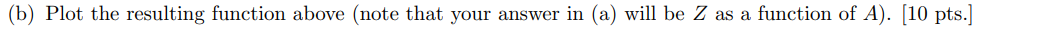
\includegraphics[scale = 0.5]{1b.png}
\end{figure}

Plotting Equation \ref{za}, we get:

\begin{figure}[H]
    \centering
    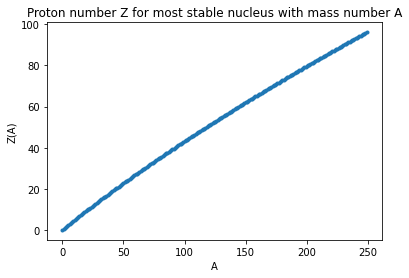
\includegraphics[scale = 0.75]{Z(A).png}
\end{figure}

It resembles the plot for stable nuclei in Figure 2.13 from Martin \& Shaw, noting that $N=A-Z$:

\begin{figure}[H]
    \centering
    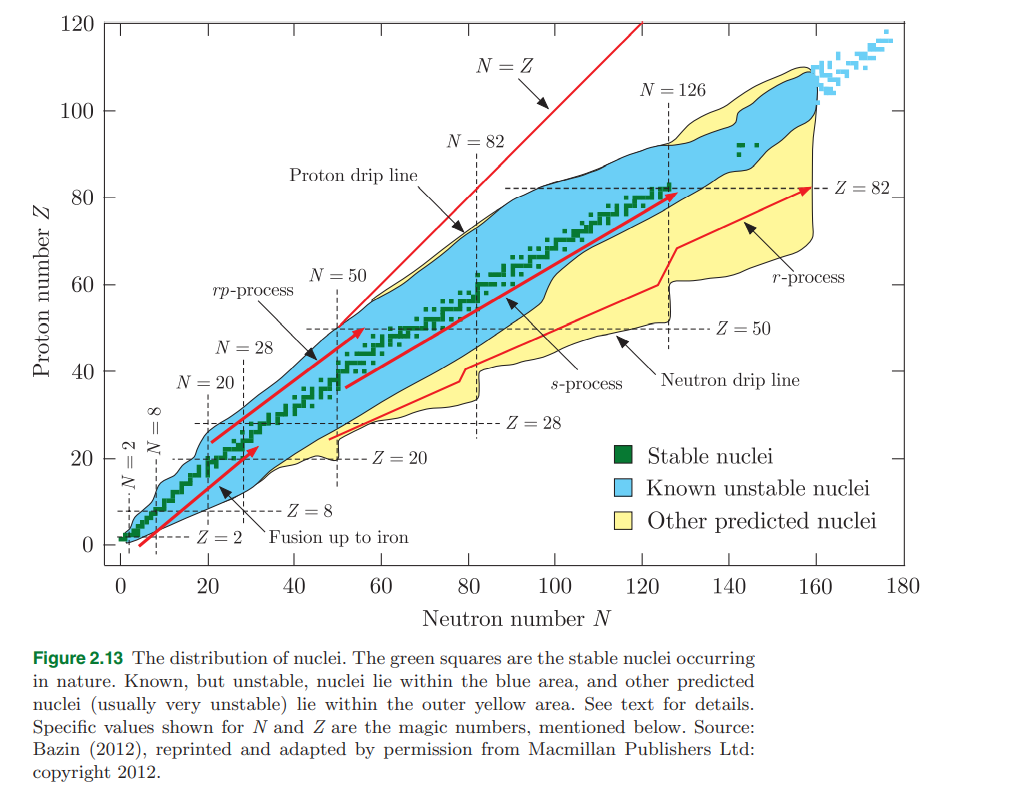
\includegraphics[scale = 0.5]{2.13.png}
\end{figure}

%==============================================================
\newpage
%==============================================================



\begin{figure}[H]
    \centering
    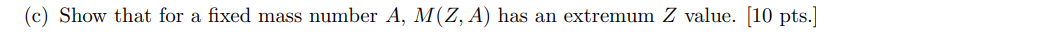
\includegraphics[scale = 0.5]{1c.png}
\end{figure}

We recall that $M(Z,A)$ is given by:

\begin{align}\label{mza}
    M(Z,A) = 
    \text{Z}(M_p + m_e) + (\text{A}-\text{Z})M_n 
    - a_v  A
    + a_s A^{2/3}
    + a_c \frac{Z(Z-1)}{A^{1/3}}
    + a_a \frac{(Z-A/2)^2}{A}
    + f_5
\end{align}

to get its extrema $Z$ value, we set $\frac{dM}{dZ} = 0$:

\begin{align}
    \frac{dM}{dZ} =
    M_p + m_e -M_n 
    + a_c \frac{2Z-1}{A^{1/3}}
    + a_a \frac{2Z-A}{A}
    =0
\end{align}

\begin{equation}\label{za2}
    \boxed{
        Z = \frac{A^{2/3}a_c + Aa_a + M_p + m_e - M_n}{2a_a + 2A^{2/3}a_c}
    }
    \end{equation}
%==============================================================
\newpage
%==============================================================


\begin{figure}[H]
    \centering
    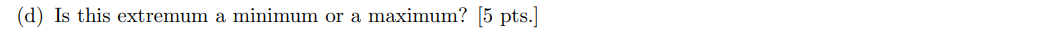
\includegraphics[scale = 0.5]{1d.png}
\end{figure}

To find out whether it is a maxima or minima, we get the second derivative with respect to $Z$:

\begin{align}
    \frac{d^2M}{dZ^2} &=
    \frac{d}{dZ}
    \left[M_p + m_e -M_n 
    + a_c \frac{2Z-1}{A^{1/3}}
    + a_a \frac{2Z-A}{A}\right]\\
    \frac{d^2M}{dZ^2} &=
     a_c \frac{2}{A^{1/3}}
    + a_a \frac{2}{A}
    > 0
\end{align}

\begin{mdframed}
    Since the second derivative will always be positive ($A$ is always positive, and the $a_i$ coeffiecients are positive as well), then the extremum is a minimum.
\end{mdframed}
%==============================================================
\newpage
%==============================================================



\begin{figure}[H]
    \centering
    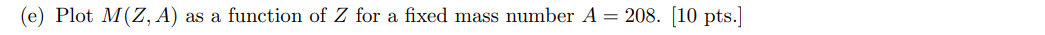
\includegraphics[scale = 0.5]{1e.png}
\end{figure}

Plotting Equation \ref{mza} for $A=208$, we have:


\begin{figure}[H]
    \centering
    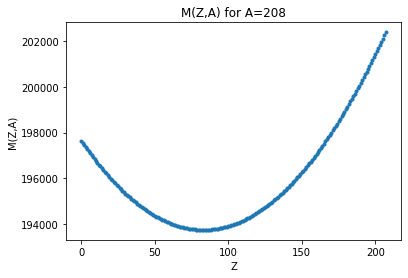
\includegraphics[scale = 0.75]{M(Z,A).png}
\end{figure}
%==============================================================
\newpage
%==============================================================




\begin{figure}[H]
    \centering
    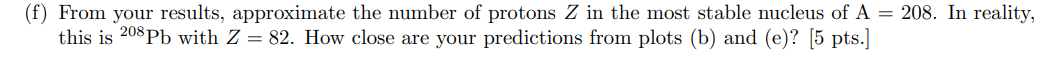
\includegraphics[scale = 0.5]{1f.png}
\end{figure}

In the following plots, $Z=82$ and/or $A=208$ is presented in the dashed lines:

\begin{figure}[H]
    \centering
    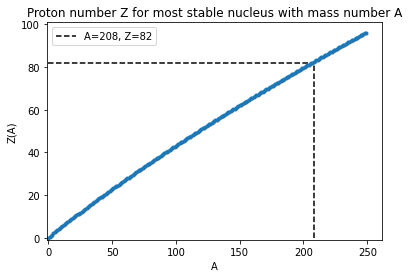
\includegraphics[scale = 0.75]{Z(A) with label.png}
\end{figure}

In the figure above, it shows that $Z=82$ and $A=208$ intersect along the plot, meaning it is a stable pair. Given that it is the most stable nucleus, this also shows the highest binding energy when plotted:

\begin{figure}[H]
    \centering
    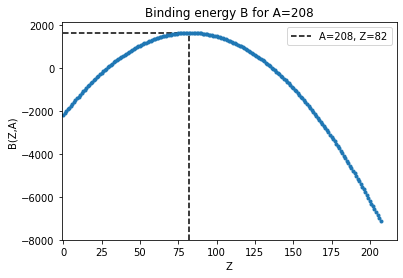
\includegraphics[scale = 0.75]{binding energy lead with label.png}
\end{figure}

Highlighting it at the plot of $M(Z,A)$:

\begin{figure}[H]
    \centering
    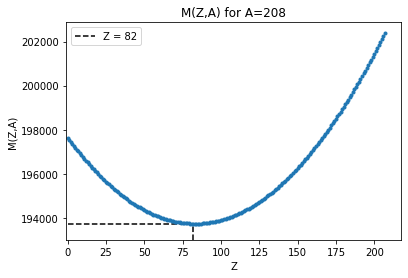
\includegraphics[scale = 0.75]{M(Z,A) with label.png}
\end{figure}

In the figure above, $Z=82$ lies at/close to the minima of the plot. This makes sense, as in the equation for binding energy, the highest binding energy (which gives the most stable nucleus) may be obtained for lower values of $M(Z,A)$.

We may also find that using previous equations with $A=208$, $Z=82$ may be almost obtained. Using Equation \ref{za}, we obtain $Z=82.46674080645812$ (meaning it is the proton number for the most stable nucleus). Using Equation \ref{za2}, we obtain $Z=82.46341480094144$ (meaning it has the lowest $M(Z,A)$).

My python code for the plots and computations are available at\newline \underline{https://colab.research.google.com/drive/1lrSsf7ZJqOBmzF7LExekYsIC9AZipV4T?usp=sharing}
%==============================================================
\newpage
%==============================================================
%we then note that we can switch up the order of differentiation:

%\begin{align*}
%    \gamma^{\nu}\gamma^{\mu} \partial_{\nu}\partial_{\mu} = \gamma^{\mu}\gamma^{\nu} \partial_{\mu}\partial_{\nu}\\
%    2\gamma^{\nu}\gamma^{\mu} \partial_{\nu}\partial_{\mu} = \gamma^{\mu}\gamma^{\nu} \partial_{\mu}\partial_{\nu} +  \gamma^{\nu}\gamma^{\mu} \partial_{\nu}\partial_{\mu}\\
%\end{align*}


%==============================================================
\newpage
%==============================================================

\begin{figure}[H]
    \centering
    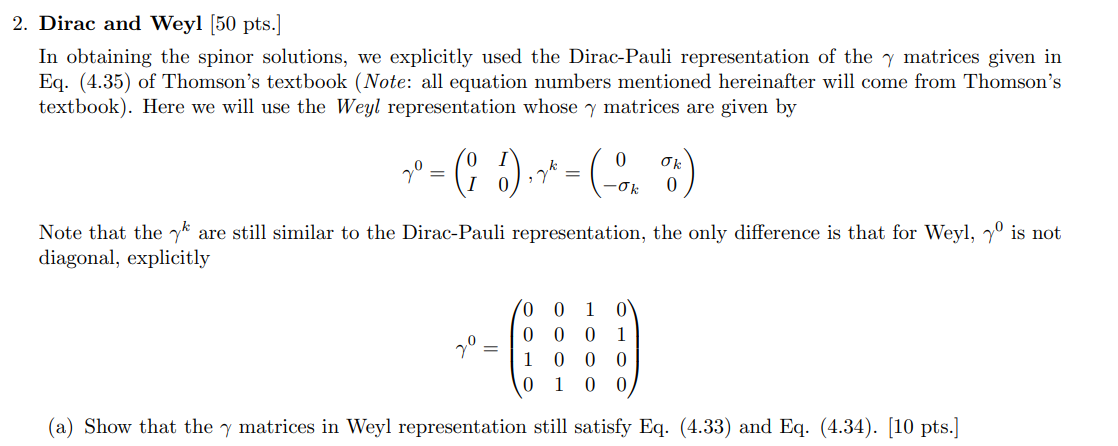
\includegraphics[scale = 0.5]{2a.png}
\end{figure}

\underline{Equation 4.33}

Equation 4.33 reads:

\begin{align*}
    \{\gamma^{\mu},\gamma^{\nu}\} \equiv 
    \gamma^{\mu}\gamma^{\nu} + \gamma^{\nu}\gamma^{\mu}
    =
    2g^{\mu\nu}
    \tag*{(4.33)}
\end{align*}

this shows the identity relations and anticommutation relation:

\begin{align}
    (\gamma^{0})^2 &= I\\
    (\gamma^{k})^2 &= -I\\
    \gamma^{\mu}\gamma^{\nu} &= -\gamma^{\nu}\gamma^{\mu}\;\text{ for } \mu \neq \nu
\end{align}

%==============================================================

\underline{\underline{$(\gamma^0)^2$}}

\begin{align}
    (\gamma^0)^2 &\stackrel{?}{=} I\\
    (\gamma^0)^2 &= \begin{pmatrix}
        0 & 0 & 1 & 0\\
        0 & 0 & 0 & 1\\
        1 & 0 & 0 & 0\\
        0 & 1 & 0 & 0\\
    \end{pmatrix}
    \begin{pmatrix}
        0 & 0 & 1 & 0\\
        0 & 0 & 0 & 1\\
        1 & 0 & 0 & 0\\
        0 & 1 & 0 & 0\\
    \end{pmatrix}\\
    (\gamma^0)^2 &=
    \begin{pmatrix}1&0&0&0\\ 0&1&0&0\\ 0&0&1&0\\ 0&0&0&1\end{pmatrix}
\end{align}

\begin{equation}
\boxed{
    (\gamma^0)^2 = I
}
\end{equation}

%==============================================================

\underline{\underline{$\gamma^{\mu}\gamma^{\nu} = -\gamma^{\nu}\gamma^{\mu}$}}

$\mu = 0$, $\nu = 1$

\begin{align}
    \gamma^{0}\gamma^{1} &\stackrel{?}{=} -\gamma^{1}\gamma^{0}\\
    \begin{pmatrix}
        0&0&1&0\\ 
        0&0&0&1\\ 
        1&0&0&0\\ 
        0&1&0&0
    \end{pmatrix}
        \begin{pmatrix}0&0&0&1\\    0&0&1&0\\    0&-1&0&0\\    -1&0&0&0\end{pmatrix} &\stackrel{?}{=}-\begin{pmatrix}0&0&0&1\\      0&0&1&0\\     0&-1&0&0\\      -1&0&0&0\end{pmatrix}\begin{pmatrix}0&0&1&0\\      0&0&0&1\\      1&0&0&0\\      0&1&0&0\end{pmatrix}\\
    \begin{pmatrix}0&-1&0&0\\ -1&0&0&0\\ 0&0&0&1\\ 0&0&1&0\end{pmatrix} &= \begin{pmatrix}0&-1&0&0\\ -1&0&0&0\\ 0&0&0&1\\ 0&0&1&0\end{pmatrix}\\
\end{align}

\begin{equation}
\boxed{
    \gamma^{0}\gamma^{1} = -\gamma^{1}\gamma^{0}
}
\end{equation}

$\mu = 0$, $\nu = 2$

\begin{align}
    \gamma^{0}\gamma^{2} &\stackrel{?}{=} -\gamma^{2}\gamma^{0}\\
    \begin{pmatrix}0&0&1&0\\     0&0&0&1\\     1&0&0&0\\     0&1&0&0\end{pmatrix}\begin{pmatrix}0&0&0&-i\\     0&0&i&0\\     0&i&0&0\\     -i&0&0&0\end{pmatrix} &\stackrel{?}{=}-\begin{pmatrix}0&0&0&-i\\       0&0&i&0\\      0&i&0&0\\       -i&0&0&0\end{pmatrix}\begin{pmatrix}0&0&1&0\\       0&0&0&1\\       1&0&0&0\\       0&1&0&0\end{pmatrix}\\
    \begin{pmatrix}0&i&0&0\\ -i&0&0&0\\ 0&0&0&-i\\ 0&0&i&0\end{pmatrix} &= \begin{pmatrix}0&i&0&0\\ -i&0&0&0\\ 0&0&0&-i\\ 0&0&i&0\end{pmatrix}\\
\end{align}

\begin{equation}
\boxed{
    \gamma^{0}\gamma^{2} = -\gamma^{2}\gamma^{0}
}
\end{equation}

$\mu = 0$, $\nu = 3$

\begin{align}
    \gamma^{0}\gamma^{3} &\stackrel{?}{=} -\gamma^{3}\gamma^{0}\\
    \begin{pmatrix}0&0&1&0\\      0&0&0&1\\      1&0&0&0\\      0&1&0&0\end{pmatrix}\begin{pmatrix}0&0&1&0\\      0&0&0&-1\\      -1&0&0&0\\      0&1&0&0\end{pmatrix} &\stackrel{?}{=}-\begin{pmatrix}0&0&1&0\\        0&0&0&-1\\       -1&0&0&0\\        0&1&0&0\end{pmatrix}\begin{pmatrix}0&0&1&0\\        0&0&0&1\\        1&0&0&0\\        0&1&0&0\end{pmatrix}\\
    \begin{pmatrix}-1&0&0&0\\ 0&1&0&0\\ 0&0&1&0\\ 0&0&0&-1\end{pmatrix} &= \begin{pmatrix}-1&0&0&0\\ 0&1&0&0\\ 0&0&1&0\\ 0&0&0&-1\end{pmatrix}\\
\end{align}

\begin{equation}
\boxed{
    \gamma^{0}\gamma^{3} = -\gamma^{3}\gamma^{0}
}
\end{equation}
%https://physics.stackexchange.com/questions/394193/proof-of-the-anti-commutation-relation-for-gamma-matrices-from-dirac-equation
%==============================================================

\underline{Equation 4.34}

Equation 4.34 reads:

\begin{align*}
    \gamma^{0\dagger} = \gamma^{0}\;
    \text{ and }
    \; \gamma^{k\dagger} = -\gamma^{k}
    \tag*{(4.34)}
\end{align*}

since the Weyl representation only differs for $\gamma^0$, we only verify the first equality in the equation:

\begin{align}
    \gamma^{0\dagger} &\stackrel{?}{=} \gamma^{0}\\
    \gamma^{0\dagger} &= \overline{(\gamma^{0})^{T}}
\end{align}

to get $\gamma^{0\dagger}$, we get the complex conjugate of the transpose of $\gamma^{0}$:

\begin{align}
    \gamma^{0} &= 
    \begin{pmatrix}
        0 & 0 & 1 & 0\\
        0 & 0 & 0 & 1\\
        1 & 0 & 0 & 0\\
        0 & 1 & 0 & 0\\
    \end{pmatrix}\\
    (\gamma^{0})^{T} &=
    \begin{pmatrix}
        0 & 0 & 1 & 0\\
        0 & 0 & 0 & 1\\
        1 & 0 & 0 & 0\\
        0 & 1 & 0 & 0\\
    \end{pmatrix}^T\\
    (\gamma^{0})^{T} &=
    \begin{pmatrix}
        0 & 0 & 1 & 0\\
        0 & 0 & 0 & 1\\
        1 & 0 & 0 & 0\\
        0 & 1 & 0 & 0\\
    \end{pmatrix}\\
\end{align}

since all elements do not have a complex part, we then have:

\begin{align}
    \overline{(\gamma^{0})^{T}} =
    \begin{pmatrix}
        0 & 0 & 1 & 0\\
        0 & 0 & 0 & 1\\
        1 & 0 & 0 & 0\\
        0 & 1 & 0 & 0\\
    \end{pmatrix} = \gamma^{0\dagger}\\
\end{align}

\begin{mdframed}
    The obtained matrix for $\gamma^{0\dagger}$ is the same as the given matrix for $\gamma^{0}$, thus we have shown that the Weyl representation still satisfies $\gamma^{0\dagger} = \gamma^{0}$ of Eq.(4.34) [and since the Dirac-Pauli representation and Weyl representation have the same $\gamma^{k}$ matrices for $k \neq 0$, the other $\gamma^{k}$ matrices of the Weyl representation also satisfy Eq.(4.34)].
\end{mdframed}
%==============================================================
\newpage
%==============================================================



\begin{figure}[H]
    \centering
    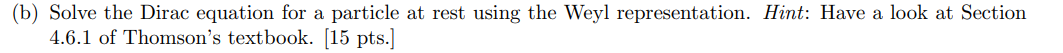
\includegraphics[scale = 0.5]{2b.png}
\end{figure}

Following 4.6.1 of Thomson, the free-particle wavefunction for a particle at rest ($\mathbf{p=0}$) is given by:

\begin{align}
    \psi &= u(E,0) e^{-iEt}\\
    E \gamma^{0}u &= mu
\end{align}

using the new $\gamma^0$ from the Weyl representation, we have:

\begin{align}
    E
    \begin{pmatrix}
        0 & 0 & 1 & 0\\
        0 & 0 & 0 & 1\\
        1 & 0 & 0 & 0\\
        0 & 1 & 0 & 0\\
    \end{pmatrix}
    \begin{pmatrix}
        \phi_1\\
        \phi_2\\
        \phi_3\\
        \phi_4
    \end{pmatrix}
    &=
    m
    \begin{pmatrix}
        \phi_1\\
        \phi_2\\
        \phi_3\\
        \phi_4
    \end{pmatrix}\\
\end{align}

solving for its eigenvalues $\lambda$, we have:

\begin{align}
    \begin{vmatrix}
        -\lambda & 0 & 1 & 0\\
        0 & -\lambda & 0 & 1\\
        1 & 0 & -\lambda & 0\\
        0 & 1 & 0 & -\lambda\\
    \end{vmatrix} &= 0\\
    %(1-\lambda)(1-\lambda)((-1-\lambda)(-1-\lambda)) &= 0\\
    \lambda &= 1,1,-1,-1
\end{align}

solving for the corresponding eigenvectors, we have:

\underline{$\lambda=1$}

\begin{align}
    \begin{pmatrix}
        -1 & 0 & 1 & 0\\
        0 & -1 & 0 & 1\\
        1 & 0 & -1 & 0\\
        0 & 1 & 0 & -1\\
    \end{pmatrix} 
    \begin{pmatrix}
        a\\
        b\\
        c\\
        d\\
    \end{pmatrix}
    &= 0\\
    -a + c &= 0\\
    -b - d &= 0\\
    a - c &= 0\\
    b - d &= 0\\
    \text{eigenvectors} &:
    \begin{pmatrix}
        1\\
        0\\
        1\\
        0\\
    \end{pmatrix},\;
    \begin{pmatrix}
        0\\
        1\\
        0\\
        1\\
    \end{pmatrix}
\end{align}


\underline{$\lambda=-1$}

\begin{align}
    \begin{pmatrix}
        1 & 0 & 1 & 0\\
        0 & 1 & 0 & 1\\
        1 & 0 & 1 & 0\\
        0 & 1 & 0 & 1\\
    \end{pmatrix} 
    \begin{pmatrix}
        a\\
        b\\
        c\\
        d\\
    \end{pmatrix}
    &= 0\\
    a + c &= 0\\
    b + d &= 0\\
    a + c &= 0\\
    b + d &= 0\\
    \text{eigenvectors} &:
    \begin{pmatrix}
        -1\\
        0\\
        1\\
        0\\
    \end{pmatrix},\;
    \begin{pmatrix}
        0\\
        -1\\
        0\\
        1\\
    \end{pmatrix}
\end{align}

The first two eigenvectors have positive energy eigenvalues ($E=+m$), whilst the latter two have negative energy eigenvalues($E=-m$). Along with normalization constant $N$, we thus have:

\begin{align}
    u_1 =  N\begin{pmatrix}
        1\\
        0\\
        1\\
        0\\
    \end{pmatrix},\;
    u_2 = N\begin{pmatrix}
        0\\
        1\\
        0\\
        1\\
    \end{pmatrix},\;
    u_3 = N\begin{pmatrix}
        -1\\
        0\\
        1\\
        0\\
    \end{pmatrix},\;
    u_4 = N\begin{pmatrix}
        0\\
        -1\\
        0\\
        1\\
    \end{pmatrix},\;
\end{align}

\begin{equation}
\boxed{
    \psi_1 =  N\begin{pmatrix}
        1\\
        0\\
        1\\
        0\\
    \end{pmatrix}e^{-imt},\;
    \psi_2 = N\begin{pmatrix}
        0\\
        1\\
        0\\
        1\\
    \end{pmatrix}e^{-imt},\;
    \psi_3 = N\begin{pmatrix}
        -1\\
        0\\
        1\\
        0\\
    \end{pmatrix}e^{+imt},\;
    \psi_4 = N\begin{pmatrix}
        0\\
        -1\\
        0\\
        1\\
    \end{pmatrix}e^{+imt},\;
}
\end{equation}
%\begin{pmatrix}0&0&1&0\\ 0&0&0&1\\ 1&0&0&0\\ 0&1&0&0\end{pmatrix}:\quad \begin{pmatrix}1\\ 0\\ 1\\ 0\end{pmatrix}, \begin{pmatrix}0\\ 1\\ 0\\ 1\end{pmatrix}, \begin{pmatrix}-1\\ 0\\ 1\\ 0\end{pmatrix}, \begin{pmatrix}0\\ -1\\ 0\\ 1\end{pmatrix}
%==============================================================
\newpage
%==============================================================




\begin{figure}[H]
    \centering
    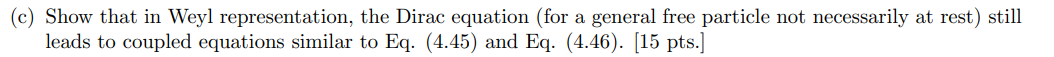
\includegraphics[scale = 0.5]{2c.png}
\end{figure}

The Dirac equation for a general free particle is given by:

\begin{align}
    (E\gamma^0 - p_x\gamma^1 - p_y\gamma^2 - p_z\gamma^3 - m)u=0
\end{align}

using the Weyl representation, this becomes:

\begin{align}
    \left[E
    \begin{pmatrix}
        0 & I\\
        I & 0\\
    \end{pmatrix}
    - 
    \begin{pmatrix}
        0 & \mathbf{\sigma \cdot p}\\
        -\mathbf{\sigma \cdot p} & 0\\
    \end{pmatrix}
    - m
    \begin{pmatrix}
        I & 0 \\
        0 & I\\
    \end{pmatrix}
    \right]u&=0\\
        \begin{pmatrix}
            -mI & EI - \mathbf{\sigma \cdot p}\\
            EI + \mathbf{\sigma \cdot p} & -mI
        \end{pmatrix}
        \begin{pmatrix}
            u_A\\
            u_B
        \end{pmatrix}
        &=
        0
        \\
\end{align}

for the coupled equations, we have:

\begin{align}
    -mI u_A + (EI-\mathbf{\sigma \cdot p}) u_B &= 0 \\
    (EI + \mathbf{\sigma \cdot p}) u_A - mI u_B &= 0\\
\end{align}

\begin{equation}
    \boxed{
    \begin{aligned}
    u_B &= \frac{m u_A}{E-\mathbf{(\sigma \cdot p)}}\\
    u_A &= \frac{m u_B}{E + \mathbf{(\sigma \cdot p)}}
    \end{aligned}
    }
\end{equation}

expanding everything in matrices, we have:

\begin{align}\biggl[
    \begin{pmatrix}
        0 & 0 & E & 0\\
        0 & 0 & 0 & E\\
        E & 0 & 0 & 0\\
        0 & E & 0 & 0\\
    \end{pmatrix}
    -
    \begin{pmatrix}
        0 & 0 & 0 & p_x\\    
        0 & 0 & p_x & 0\\    
        0 & -p_x & 0 & 0\\    
        -p_x & 0 & 0 & 0
    \end{pmatrix}
    -
    \begin{pmatrix}
        0 & 0 & 0 & -ip_y\\     
        0 & 0 & ip_y & 0\\     
        0 & ip_y & 0 & 0\\     
        -ip_y & 0 & 0 & 0
    \end{pmatrix}\\
    -
    \begin{pmatrix}
        0 & 0 & p_z & 0\\      
        0 & 0 & 0 & -p_z\\      
        -p_z & 0 & 0 & 0 \\      
        0 & p_z & 0 & 0
    \end{pmatrix}
    -
    \begin{pmatrix}
        m & 0 & 0 & 0\\
        0 & m & 0 & 0\\
        0 & 0 & m & 0\\
        0 & 0 & 0 & m\\
    \end{pmatrix}
\biggr]
\begin{pmatrix}
    u_{A1}\\
    u_{A2}\\
    u_{B1}\\
    u_{B2}
\end{pmatrix}    
=0\\
\begin{pmatrix}
    -m & 0 & E-p_z & -p_x+ip_y\\
    0 & -m & -p_x-ip_y & E+p_z\\
    E+p_z & p_x-ip_y & -m & 0\\
    p_x+ip_y & E-p_z & 0 & -m 
\end{pmatrix}
\begin{pmatrix}
    u_{A1}\\
    u_{A2}\\
    u_{B1}\\
    u_{B2}
\end{pmatrix}    
=0\\
\end{align}

the corresponding equations we have are:

\begin{align}
    -mu_{A1} + (E-p_z)u_{B1} + (-p_x+ip_y)u_{B2} &= 0\\
    -mu_{A2} + (-p_x-ip_y)u_{B1} + (E + p_z) u_{B2} &= 0\\
    (E+p_z)u_{A1} + (p_x-ip_y)u_{A2} + (-m)u_{B1} &= 0\\
    (p_x+ip_y)u_{A1} (E-p_z)u_{A2} + (-m)u_{B2} &= 0
\end{align}

we note that at least one of the elements of $u_A$ ($u_{A1}$ and $u_{A2}$) and $u_B$ ($u_{B1}$ and $u_{B2}$) are mixed in each equation.

%\begin{equation}
 %   \boxed{
 %   \begin{aligned}
 %      
 %   \end{aligned}
 %   }
 %\end{equation}
 
%==============================================================
\newpage
%==============================================================



\begin{figure}[H]
    \centering
    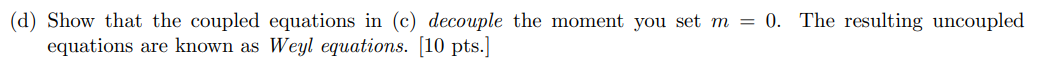
\includegraphics[scale = 0.5]{2d.png}
\end{figure}

the coupled equations earlier show that:

\begin{align}
    u_B &= \frac{m u_A}{E-\mathbf{(\sigma \cdot p)}}\\
    u_A &= \frac{m u_B}{E + \mathbf{(\sigma \cdot p)}}
\end{align}

\begin{align}
    (E-\mathbf{(\sigma \cdot p)})u_B &= m u_A\\
    (E + \mathbf{(\sigma \cdot p)})u_A &= m u_B
\end{align}

setting $m=0$, we get:

\begin{equation}
    \boxed{
    \begin{aligned}
        [E-\mathbf{(\sigma \cdot p)}] u_B &= 0\\
        [E + \mathbf{(\sigma \cdot p)}]u_A &= 0
    \end{aligned}
    }
 \end{equation}

 the equations have decoupled. We can also see this in the expanded versions of the equation when $m=0$:

 \begin{align}
    (E-p_z)u_{B1} + (-p_x+ip_y)u_{B2} &= 0\\
   (-p_x-ip_y)u_{B1} + (E + p_z) u_{B2} &= 0\\
    (E+p_z)u_{A1} + (p_x-ip_y)u_{A2} &= 0\\
    (p_x+ip_y)u_{A1} (E-p_z)u_{A2} &= 0
\end{align}


%==============================================================
\newpage
%==============================================================






%we note that in our earlier solution evaluating $\gamma^{0}\gamma^{0}\gamma^{0}$, we found that $\gamma^{0}\gamma^{0} = \begin{pmatrix}1&0&0&0\\ 0&1&0&0\\ 0&0&1&0\\ 0&0&0&1\end{pmatrix} = I$. Thus we can rewrite the LHS of the equation as:

%\begin{align*}
%    -\gamma^{k} = -I\gamma^{k}\\
%    -\gamma^{k} = -\gamma^{0}\gamma^{0}\gamma^{k}
%\end{align*}

%we can rewrite the RHS of the equation as:

%\begin{align*}
%    \gamma^{0}\gamma^{k}\gamma^{0} = 
%\end{align*}
%==================================
\end{document}